% !TEX root =  ../supplementary.tex

\section{Parameter Estimates from the Joint Model Fitted to the PRIAS Dataset}
\label{sec:param_estimates_jm_fit_prias}

We fit a joint model to the PRIAS dataset using the R package \textbf{JMbayes} \citep{rizopoulosJMbayes}. The corresponding posterior parameter estimates are shown in Table~\ref{tab:DRE_long} (longitudinal sub-model for DRE outcome), Table~\ref{tab:PSA_long} (longitudinal sub-model for PSA outcome) and Table~\ref{tab:DRE_PSA_survival} (relative risk sub-model). The parameter estimates for the variance-covariance matrix $\boldsymbol{D}$ from the longitudinal sub-model are shown in the following Table~\ref{tab:D_matrix}:
\begin{table}[!htb]
\begin{center}
\caption{Estimated variance-covariance matrix $\boldsymbol{D}$ of the random effects ${\boldsymbol{b}=(b_{0d},b_{1d},b_{0p}, b_{1p}, b_{2p}, b_{3p}, b_{4p})}$ (see \ref{subsec:model_def}) from the joint model fitted to the PRIAS dataset. The variances of the random effects are highlighted along the diagonal of the variance-covariance matrix.}
\label{tab:D_matrix}
\begin{tabular}{lrrrrrrr}
\Hline
Random Effects    & $b_{0d}$    & $b_{1d}$    & $b_{0p}$    & $b_{1p}$   & $b_{2p}$   & $b_{3p}$   & $b_{4p}$    \\
\hline
$b_{0d}$ & \cellcolor{black}\textcolor{white}{7.55}  & -0.56 & -0.18 & 0.08 & 0.084 & 0.003 & -0.019 \\
$b_{1d}$ & -0.564 & \cellcolor{black}\textcolor{white}{1.379}  & 0.081  & 0.119 & 0.165 & 0.266 & 0.219  \\
\hline
$b_{0p}$ & -0.182 & 0.081  & \cellcolor{black}\textcolor{white}{0.208}  & 0.031 & 0.034 & 0.068 & 0.014  \\
$b_{1p}$ & 0.075  & 0.119  & 0.031  & \cellcolor{black}\textcolor{white}{0.224} & 0.109 & 0.158 & 0.088  \\
$b_{2p}$ & 0.084  & 0.165  & 0.034  & 0.109 & \cellcolor{black}\textcolor{white}{0.293} & 0.324 & 0.238  \\
$b_{3p}$ & 0.003  & 0.266  & 0.068  & 0.158 & 0.324 & \cellcolor{black}\textcolor{white}{0.480} & 0.312  \\
$b_{4p}$ & -0.019 & 0.219  & 0.014  & 0.088 & 0.238 & 0.312 & \cellcolor{black}\textcolor{white}{0.290}  \\
\hline
\end{tabular}
\end{center}
\end{table}

For the DRE mixed effects sub-model (see Equation \ref{eq:long_model_dre}) parameter estimates, in Table~\ref{tab:DRE_long} we can see that the age of the patient trivially affects the baseline log odds of obtaining a DRE measurement larger than T1c. In Figure~\ref{fig:fitted_marginal_dre} we present the marginal evolution of log odds of obtaining a DRE larger than T1c, and the corresponding marginal probability, over a period of 10 years for a hypothetical AS patient who is included in AS at the age of 70 years. In addition, we present plots of observed DRE versus fitted probabilities of obtaining a DRE measurement larger than T1c, for nine randomly selected patients in Figure~\ref{fig:fitted_9subject_dre}.

\begin{table}[!htb]
\begin{center}
\caption{Estimated mean and 95\% credible interval for the parameters of the longitudinal sub-model (see Equation \ref{eq:long_model_dre}) for the DRE outcome.}
\label{tab:DRE_long}
\begin{tabular}{lrrrrr}
\Hline
Variable                         & Mean & Std. Dev & 2.5\%  & 97.5\% & P     \\
\hline
(Intercept)                      & -4.017   & 0.136 & -4.270  & -3.763 & \textless0.001     \\
$(\mbox{Age} - 70)$                      & 0.058    & 0.009 & 0.041  & 0.075  & \textless0.001     \\
$(\mbox{Age} - 70)^2$ & -0.001   & 0.001 & -0.003 & 0.000      & 0.076 \\
visitTimeYears                   & -0.604   & 0.095 & -0.794 & -0.437 & \textless0.001    \\
\hline
\end{tabular}
\end{center}
\end{table}

\begin{figure}[!htb]
\centerline{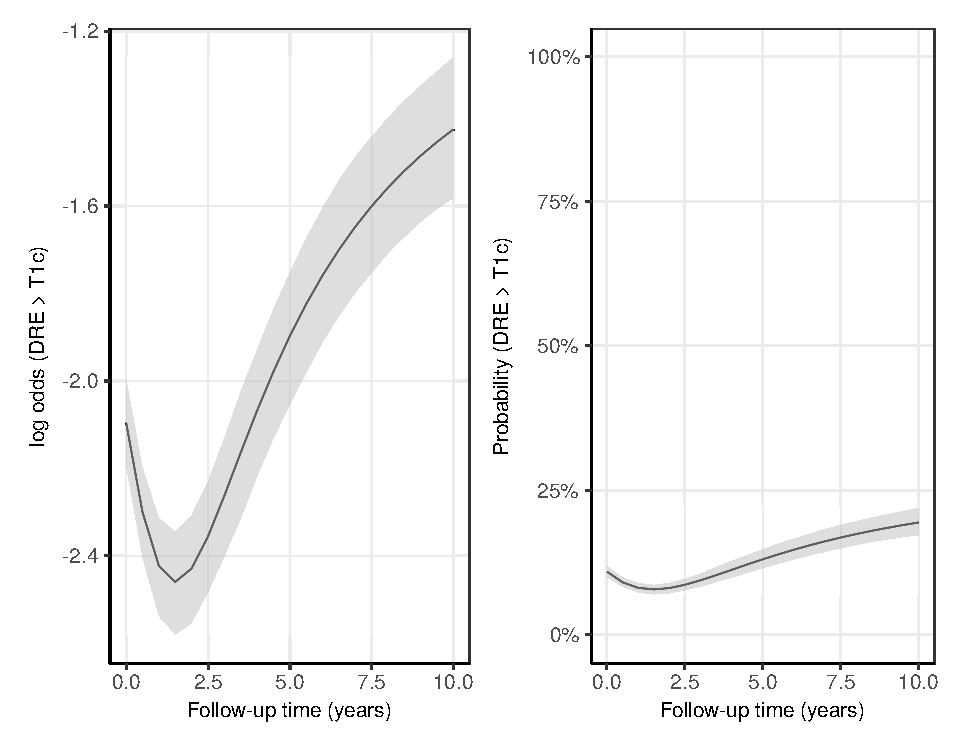
\includegraphics[width=\columnwidth]{images/marginal_dre_both.eps}}
\caption{Fitted marginal evolution of the log odds of obtaining a DRE larger than T1c, and the corresponding marginal probability, with 95\% credible interval. These results are for a hypothetical AS patient who is included in AS at the age of 70 years.}
\label{fig:fitted_marginal_dre}
\end{figure}

\begin{figure}[!htb]
\centerline{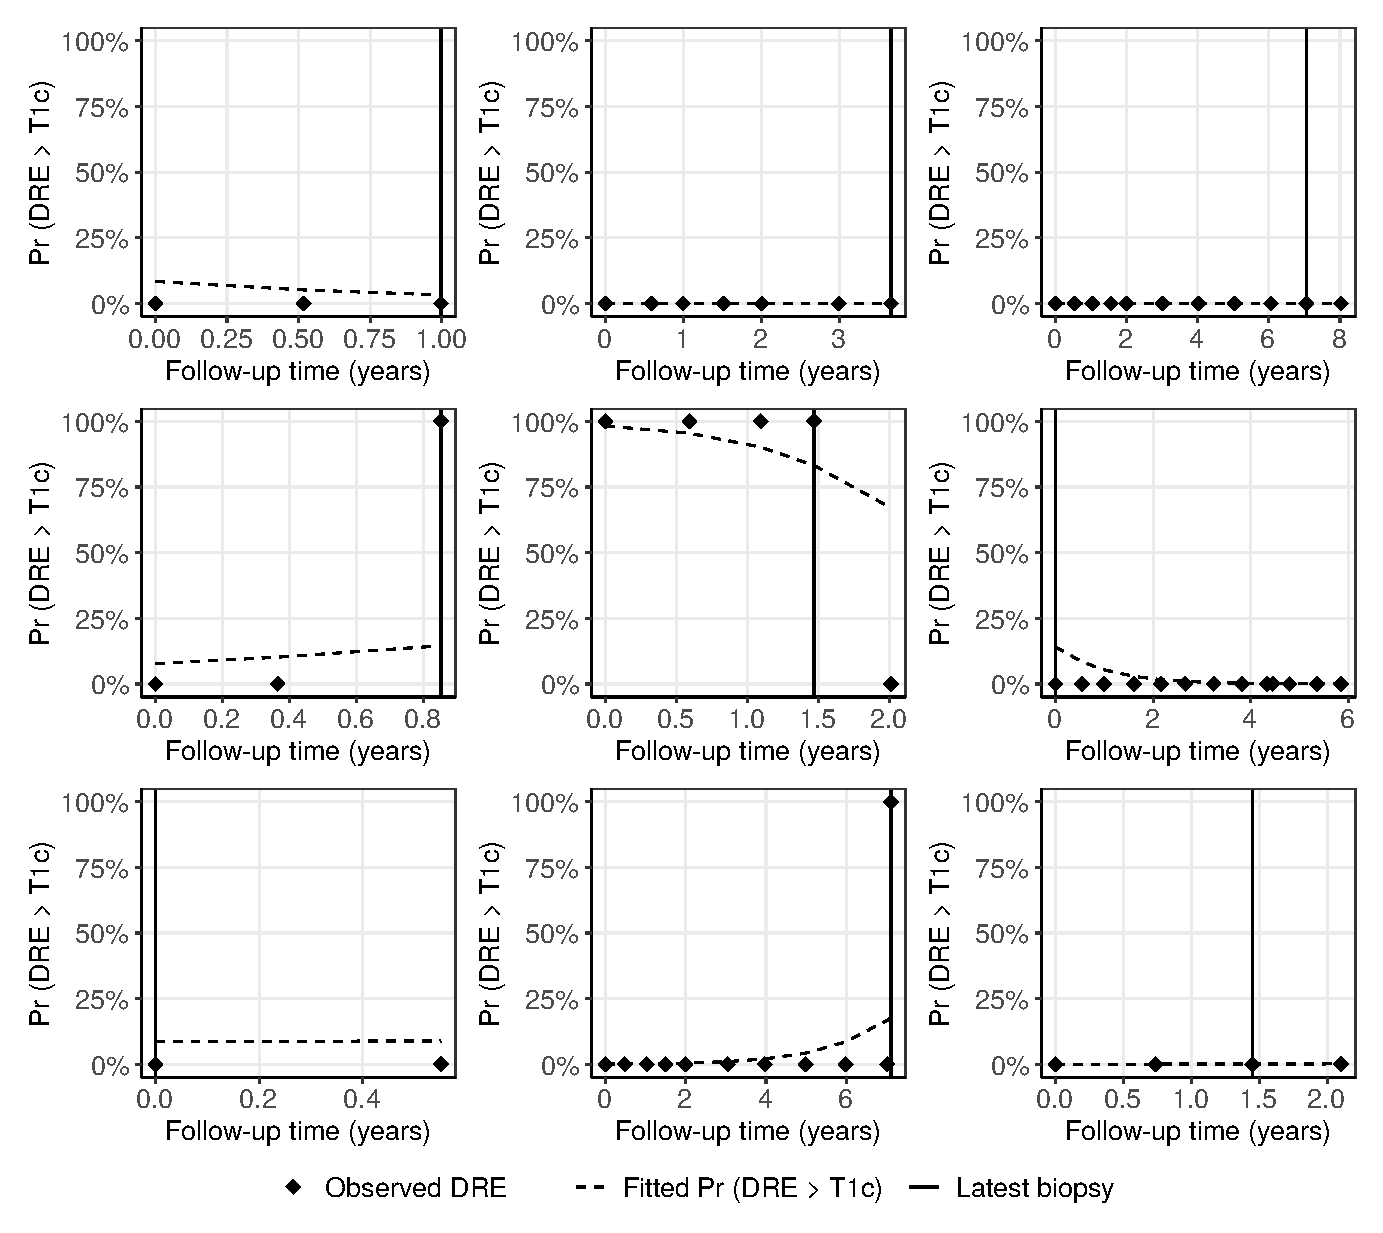
\includegraphics[width=\columnwidth]{images/fitted_9subject_dre.eps}}
\caption{Observed DRE versus fitted probabilities of obtaining a DRE measurement larger than T1c, for nine randomly selected PRIAS patients. The fitted profiles utilize information from the observed DRE measurements, PSA measurements, and time of the latest biopsy. Observed DRE measurements plotted against 0\% probability are equal to T1c. Observed DRE measurements plotted against 100\% probability are larger than T1c.}
\label{fig:fitted_9subject_dre}
\end{figure}

\clearpage

For the PSA mixed effects sub-model parameter estimates (see Equation \ref{eq:long_model_psa}), in Table~\ref{tab:PSA_long} we can see that the age of the patient trivially affects the baseline ${\log_2(\mbox{PSA} + 1)}$ measurement. Since the longitudinal evolution of ${\log_2 (\mbox{PSA} + 1)}$ measurements is modeled with non-linear terms, the interpretation of the coefficients corresponding to time is not straightforward. In lieu of the interpretation, in Figure~\ref{fig:fitted_marginal_psa} we present the fitted marginal evolution of ${\log_2 (\mbox{PSA} + 1)}$ over a period of 10 years for a hypothetical patient who is included in AS at the age of 70 years. In addition, we present plots of observed versus fitted PSA profiles for nine randomly selected patients in Figure~\ref{fig:fitted_9subject_psa}. 

\begin{table}[!htb]
\begin{center}
\caption{Estimated mean and 95\% credible interval for the parameters of the longitudinal sub-model (see Equation \ref{eq:long_model_psa}) for the PSA outcome.}
\label{tab:PSA_long}
\begin{tabular}{lrrrrr}
\Hline
Variable                         & Mean & Std. Dev & 2.5\%  & 97.5\% & P     \\
\hline
(Intercept) & 2.701 & 0.008 & 2.686  & 2.716  & \textless0.001 \\
$(\mbox{Age} - 70)$ & 0.003 & 0.001 & 0.001  & 0.005  & \textless0.001 \\
$(\mbox{Age} - 70)^2$ & -4.7 $\times 10^{-4}$     & 9.8 $\times 10^{-5}$     & -6.6 $\times 10^{-4}$ & -2.7 $\times 10^{-4}$      & \textless0.001 \\
Spline: [0.00, 0.10] years & 0.054 & 0.009 & 0.037  & 0.073  & \textless0.001 \\
Spline: [0.10, 0.70] years & 0.177 & 0.012 & 0.151  & 0.200  & \textless0.001 \\
Spline: [0.70, 4.00] years & 0.194 & 0.016 & 0.161  & 0.225  & \textless0.001 \\
Spline: [4.00, 5.42] years & 0.341 & 0.015 & 0.312  & 0.371  & \textless0.001 \\
$\sigma$ & 0.137 & 0.001 & 0.135  & 0.138  & \\
\hline
\end{tabular}
\end{center}
\end{table}

\begin{figure}[!htb]
\centerline{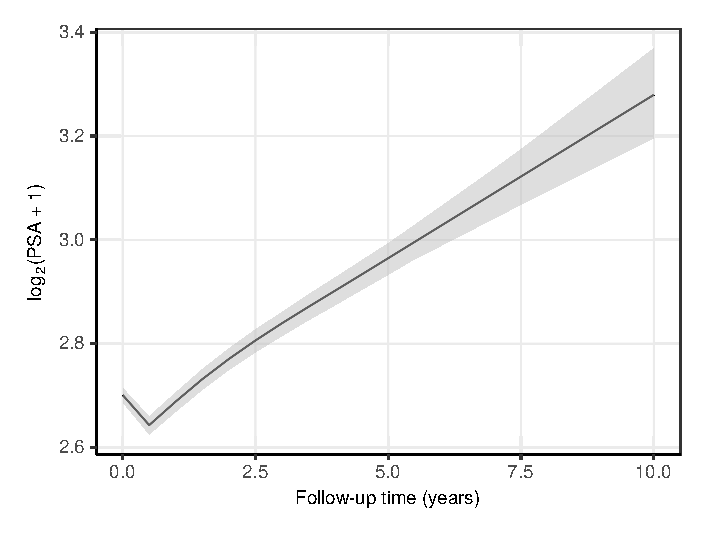
\includegraphics[width=0.7\columnwidth]{images/marginal_psa.eps}}
\caption{Fitted marginal evolution of $\log_2 (\mbox{PSA} + 1)$ measurements over a period of 10 years with 95\% credible interval, for a hypothetical patient who is included in AS at the age of 70 years.}
\label{fig:fitted_marginal_psa}
\end{figure}

\begin{figure}[!htb]
\centerline{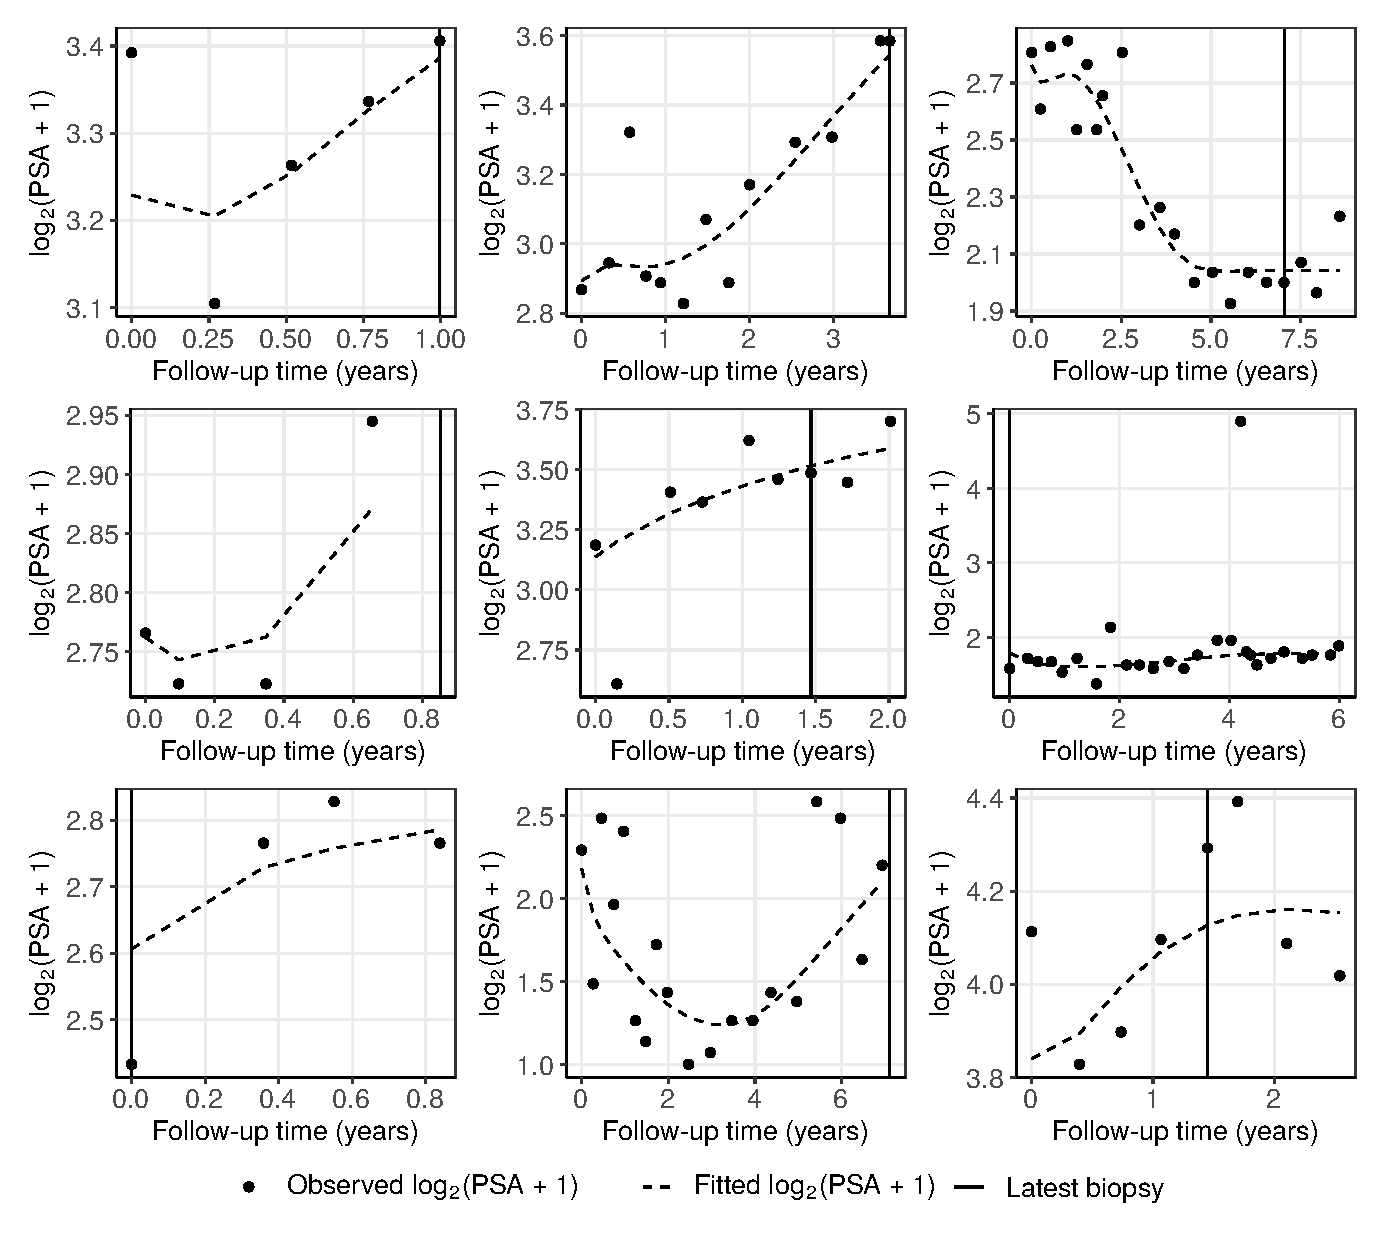
\includegraphics[width=\columnwidth]{images/fitted_9subject_psa.eps}}
\caption{Fitted versus observed ${\log_2 (\mbox{PSA} + 1)}$ profiles for nine randomly selected PRIAS patients. The fitted profiles utilize information from the observed PSA measurements, DRE measurements, and time of the latest biopsy.}
\label{fig:fitted_9subject_psa}
\end{figure}

\clearpage

For the relative risk sub-model (see Equation \ref{eq:rel_risk_model}), the parameter estimates in Table~\ref{tab:DRE_PSA_survival} show that both ${\log_2 \{\mbox{PSA} + 1\}}$ velocity,  and the log odds of having ${\mbox{DRE} > \mbox{T1c}}$  were significantly associated with the hazard of cancer progression.  

\begin{table}[!htb]
\begin{center}
\caption{Estimated mean and 95\% credible interval for the parameters of the relative risk sub-model (see Equation \ref{eq:rel_risk_model}) of the joint model fitted to the PRIAS dataset.}
\label{tab:DRE_PSA_survival}
\begin{tabular}{lrrrrr}
\Hline
Variable                      & Mean   & Std. Dev & 2.5\%  & 97.5\%                 & P              \\
\hline
$(\mbox{Age} - 70)$                      & 0.012    & 0.006 & 0.000 & 0.022  & 0.045 \\
$(\mbox{Age} - 70)^2$ & -0.001   & 0.001 & -0.002 & 0.000      & 0.095 \\
$\mbox{logit} \big\{\mbox{Pr}(\mbox{DRE} > \mbox{T1c})\big\}$                 & 0.147    & 0.017 & 0.115  & 0.183  & \textless0.001     \\
Fitted $\log_2 (\mbox{PSA} + 1)$ value            & 0.104    & 0.078 & -0.044 & 0.256  & 0.193 \\
Fitted $\log_2 (\mbox{PSA} + 1)$ velocity             & 3.396    & 0.564 & 2.376  & 4.475  & \textless0.001   \\
\hline
\end{tabular}
\end{center}
\end{table}

It is important to note that since age, ${\log_2 \{\mbox{PSA} + 1\}}$ value and velocity, and log odds of ${\mbox{DRE} > \mbox{T1c}}$ are all measured on different scales, a comparison between the corresponding parameter estimates is not easy. To this end, in Table \ref{tab:DRE_PSA_survival_easy}, we present the hazard (of cancer progression) ratio, for an increase in the aforementioned variables from their first to the third quartile. For example, an increase in log odds of DRE > T1c, from -6.650 to -4.356 (fitted first and third quartiles) corresponds to a hazard ratio of 1.402. The interpretation for the rest is similar.

\begin{table}[!htb]
\begin{center}
\caption{Hazard (of cancer progression) ratio and 95\% credible interval (CI), for an increase in the variables of relative risk sub-model, from their first quartile ($\mbox{Q}_1$) to their third quartile ($\mbox{Q}_3$). Except for age, quartiles for all other variables are based on their fitted values obtained from the joint model fitted to the PRIAS dataset.}
\label{tab:DRE_PSA_survival_easy}
\begin{tabular}{lrrr}
\Hline
Variable                      & $\mbox{Q}_1$   & $\mbox{Q}_3$ & Hazard ratio [95\% CI] \\
\hline
Age & 65 & 75 & 1.129 [1.002, 1.251] \\
$\mbox{logit} \big\{\mbox{Pr}(\mbox{DRE} > \mbox{T1c})\big\}$ & -6.650 & -4.356 & 1.402 [1.301, 1.521]\\
$\log_2 (\mbox{PSA} + 1)$ value & 2.336 & 3.053 & 1.079 [0.969, 1.201]\\
$\log_2 (\mbox{PSA} + 1)$ velocity & -0.032 & 0.161 & 1.938 [1.582, 2.372]\\
\hline
\end{tabular}
\end{center}
\end{table}



\clearpage

\subsection{Assumption of t-distributed (df=3) Error Terms}
\label{subsec:t-dist-assumption}
With regards to the choice of the distribution for the error term $\varepsilon_p$ for the PSA measurements (see Equation \ref{eq:long_model_psa}), we attempted fitting multiple joint models differing in error distribution, namely t-distribution with three, and four degrees of freedom, and a normal distribution for the error term. However, the model assumption for the error term were best met by the model with t-distribution having three degrees of freedom. The quantile-quantile plot of subject-specific residuals for the corresponding model in Panel~A of Figure~\ref{fig:qqplot}, shows that the assumption of t-distributed (df=3) errors is reasonably met by the fitted model. 

\begin{figure}[!htb]
\centerline{\includegraphics[width=\columnwidth]{images/qqplot.eps}}
\caption{Quantile-quantile plot of subject-specific residuals from the joint models fitted to the PRIAS dataset. \textbf{Panel A}: model assuming a t-distribution (df=3) for the error term $\varepsilon_p$. \textbf{Panel B}: model assuming a normal distribution for the error term $\varepsilon_p$.}
\label{fig:qqplot}
\end{figure}

\clearpage
\subsection{Predictive Performance of the Joint Model Fitted to the PRIAS dataset}
We evaluate the predictive performance of our model using two measures: the area under the receiver operating characteristic curve (AUC), and the prediction error. Given the longitudinal nature of the data at hand, in a joint model time dependent AUC and prediction errors are more relevant. More specifically, given the time of latest biopsy $t$, and history of DRE and PSA measurements up to time $s$, we are interested in a medically relevant time frame $(t, s]$, within which the occurrence of cancer progression is of interest. In the case of prostate cancer, at any point in time it is of interest to identify patients who may have obtained cancer progression in the last one year ($s-t = 1$). Using data of the patients from the PRIAS study, we calculate the AUC and prediction error (see \citet{landmarking2017} for estimation) at the following $s$: year one, year two, year three, year four, and year five (95-percentile of observed cancer progression times) of follow-up in AS. The resulting AUC, and prediction are presented in Table \ref{tab:AUC_PE}.

\begin{table}[!htb]
\begin{center}
\caption{Area under the receiver operating characteristic curves (AUC), and prediction error, with 95\% confidence interval in brackets.}
\label{tab:AUC_PE}
\begin{tabular}{r|r|r}
\Hline
Follow-up year & AUC & Prediction Error\\ 
\hline
1 & 0.651 [0.633, 0.663] & 0.055 [0.052, 0.059]\\
2 & 0.621 [0.610, 0.640] & 0.144 [0.140, 0.148]\\
3 & 0.748 [0.728, 0.770] & 0.076 [0.075, 0.078]\\
4 & 0.710 [0.691, 0.736] & 0.076 [0.072, 0.079]\\
5 & 0.592 [0.577, 0.614] & 0.107 [0.103, 0.112]\\
\hline
\end{tabular}	
\end{center}
\end{table}

%\begin{table}[!htb]
%\begin{center}
%\caption{Area under the receiver operating characteristic curves (AUC), and 95\% confidence interval in brackets. AUC's are calculated for two joint models: first one utilizing information from both DRE and PSA measurements, and second one utilizing information from only PSA measurements.}
%\label{tab : AUC}
%\begin{tabular}{rrr}
%\Hline
%Year                      & both DRE and PSA & only PSA\\ 
%\hline
%1 & 0.651 [0.633, 0.663] & 0.636 [0.626, 0.648]\\
%2 & 0.621 [0.610, 0.640] & 0.593 [0.584, 0.606]\\
%3 & 0.748 [0.728, 0.770] & 0.716 [0.699, 0.733]\\
%4 & 0.710 [0.691, 0.736] & 0.643 [0.623, 0.660]\\
%5 & 0.592 [0.577, 0.614] & 0.536 [0.517, 0.553]\\
%\hline
%\end{tabular}	
%\end{center}
%\end{table}

%\begin{table}[!htb]
%\begin{center}
%\caption{Prediction error, and 95\% confidence interval in brackets. Prediction errors are calculated for two joint models: first one utilizing information from both DRE and PSA measurements, and second one utilizing information from only PSA measurements.}
%\label{tab : PE}
%\begin{tabular}{rrr}
%\Hline
%Year                      & both DRE and PSA & only PSA\\ 
%\hline
%1 & 0.055 [0.052, 0.059] & 0.056 [0.052, 0.059]\\
%2 & 0.144 [0.140, 0.148] & 0.148 [0.145, 0.153]\\
%3 & 0.076 [0.075, 0.078] & 0.077 [0.075, 0.080]\\
%4 & 0.076 [0.072, 0.079] & 0.077 [0.073, 0.080]\\
%5 & 0.107 [0.103, 0.112] & 0.116 [0.112, 0.122]\\
%\hline
%\end{tabular}	
%\end{center}
%\end{table}